\noindent\textbf{Any}
\lstinputlisting[firstline=1,lastline=3]{transformations/set/emftvm/TestAny.atl}
\begin{figure*}[h]
\centering
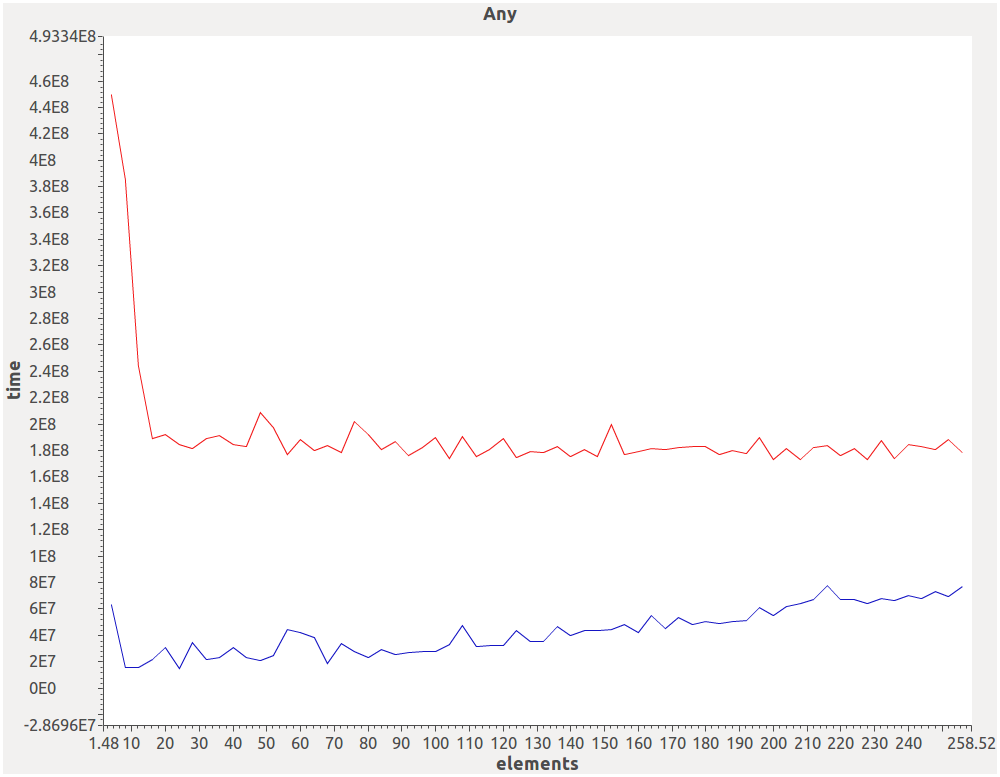
\includegraphics[width=\textwidth]{graphs/set/Any}
\end{figure*}
\pagebreak

\noindent\textbf{Collect}
\lstinputlisting[firstline=1,lastline=3]{transformations/set/emftvm/TestCollect.atl}
\begin{figure*}[h]
\centering
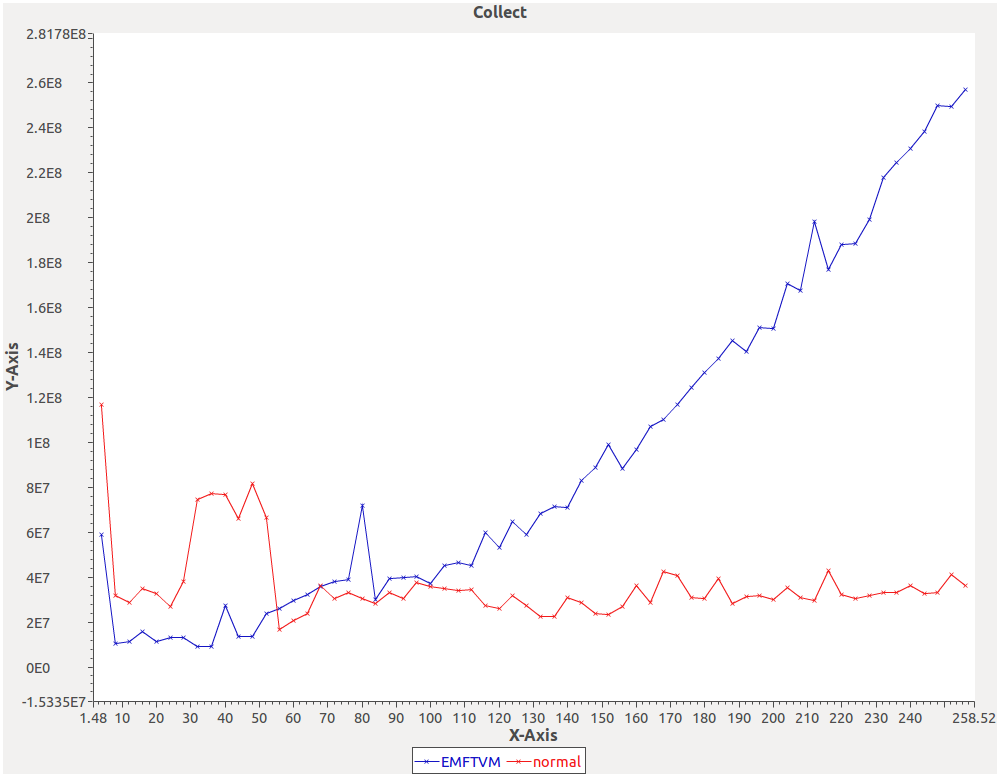
\includegraphics[width=\textwidth]{graphs/set/Collect}
\end{figure*}
\pagebreak

\noindent\textbf{EQ}
\lstinputlisting[firstline=1,lastline=3]{transformations/set/emftvm/TestEQ.atl}
\begin{figure*}[h]
\centering
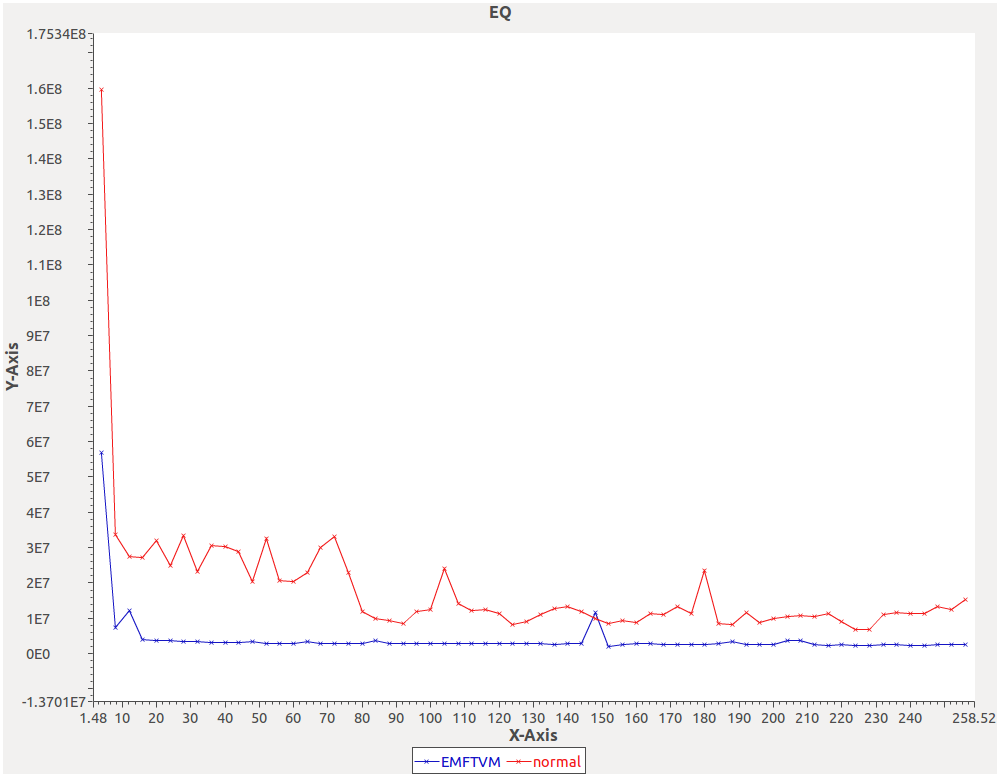
\includegraphics[width=\textwidth]{graphs/set/EQ}
\end{figure*}
\pagebreak

\noindent\textbf{Excludes}
\lstinputlisting[firstline=1,lastline=3]{transformations/set/emftvm/TestExcludes.atl}
\begin{figure*}[h]
\centering
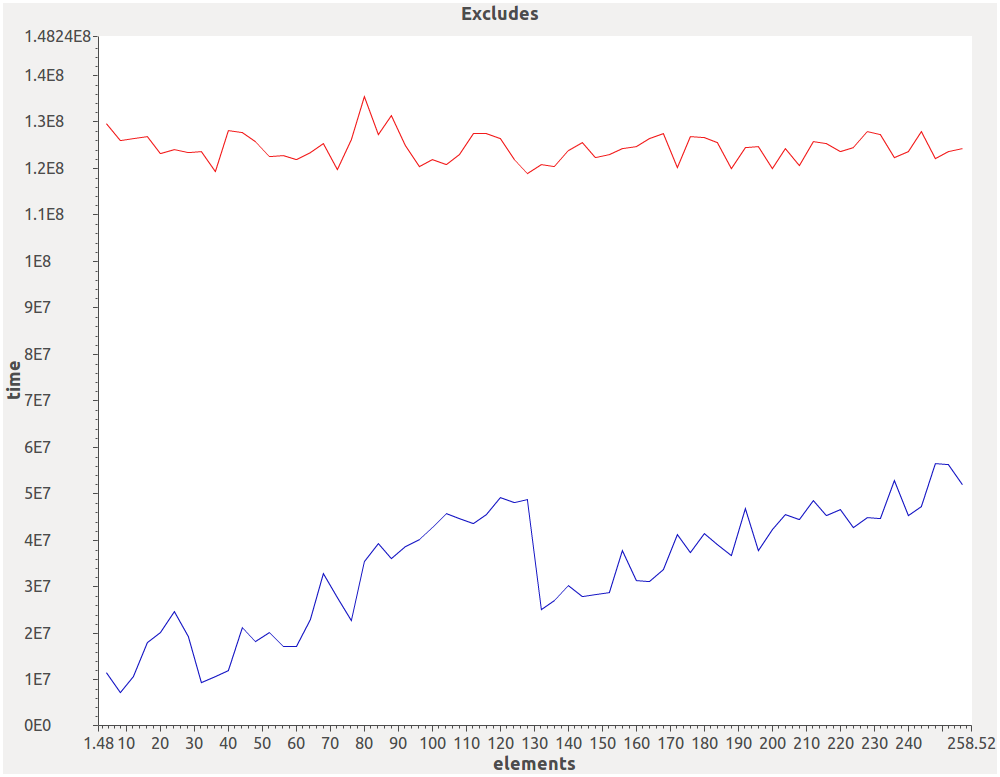
\includegraphics[width=\textwidth]{graphs/set/Excludes}
\end{figure*}
\pagebreak

\noindent\textbf{ExcludesAll}
\lstinputlisting[firstline=1,lastline=3]{transformations/set/emftvm/TestExcludesAll.atl}
\begin{figure*}[h]
\centering
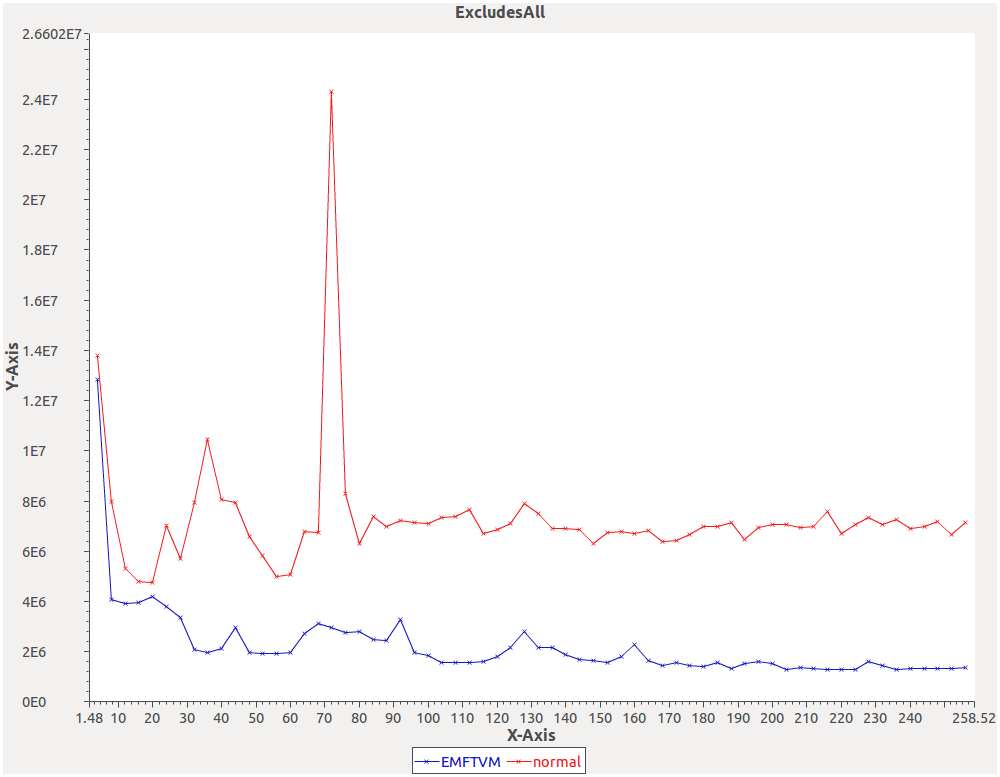
\includegraphics[width=\textwidth]{graphs/set/ExcludesAll}
\end{figure*}
\pagebreak

\noindent\textbf{Excluding}
\lstinputlisting[firstline=1,lastline=3]{transformations/set/emftvm/TestExcluding.atl}
\begin{figure*}[h]
\centering
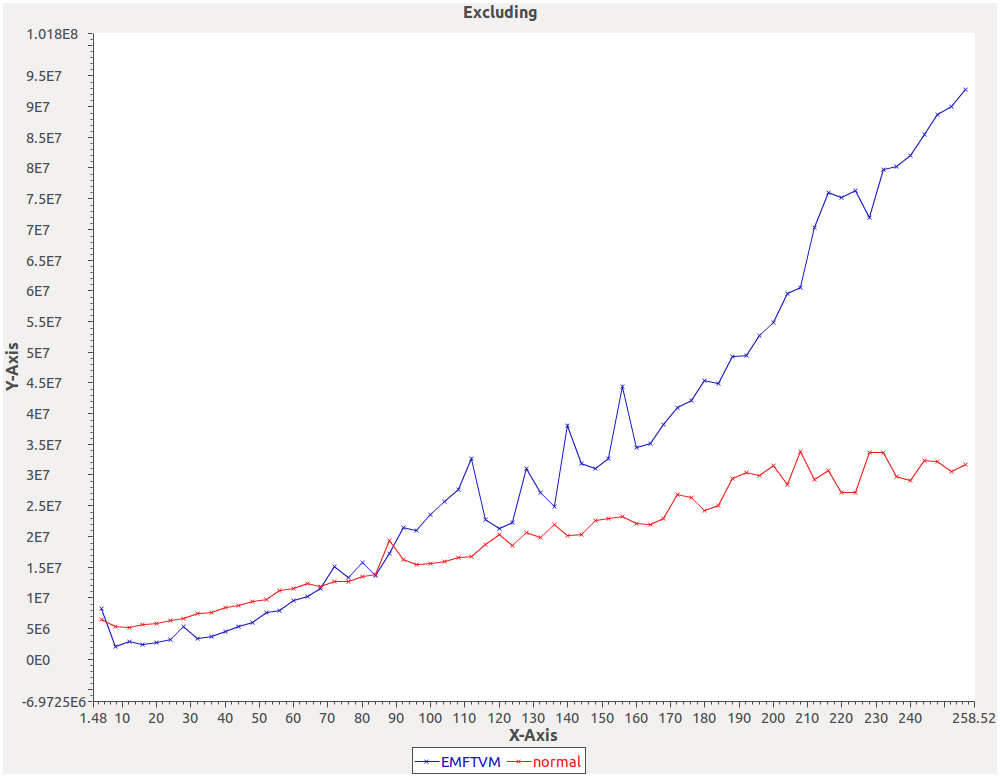
\includegraphics[width=\textwidth]{graphs/set/Excluding}
\end{figure*}
\pagebreak

\noindent\textbf{Exists}
\lstinputlisting[firstline=1,lastline=3]{transformations/set/emftvm/TestExists.atl}
\begin{figure*}[h]
\centering
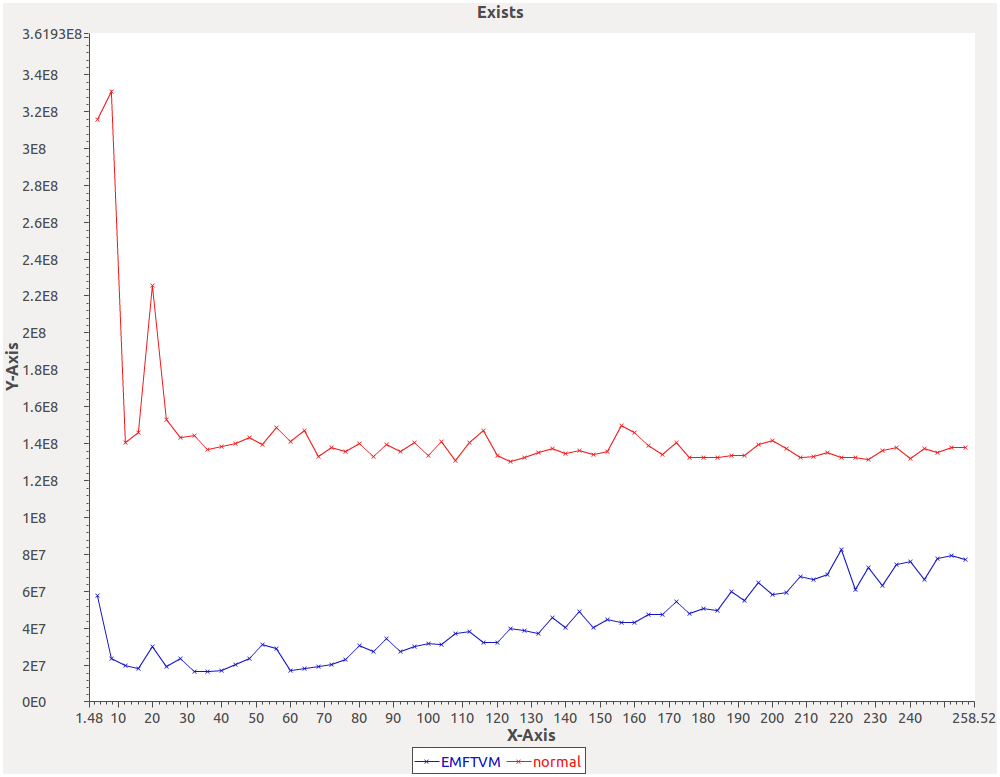
\includegraphics[width=\textwidth]{graphs/set/Exists}
\end{figure*}
\pagebreak

\noindent\textbf{Flatten}
\lstinputlisting[firstline=1,lastline=3]{transformations/set/emftvm/TestFlatten.atl}
\begin{figure*}[h]
\centering
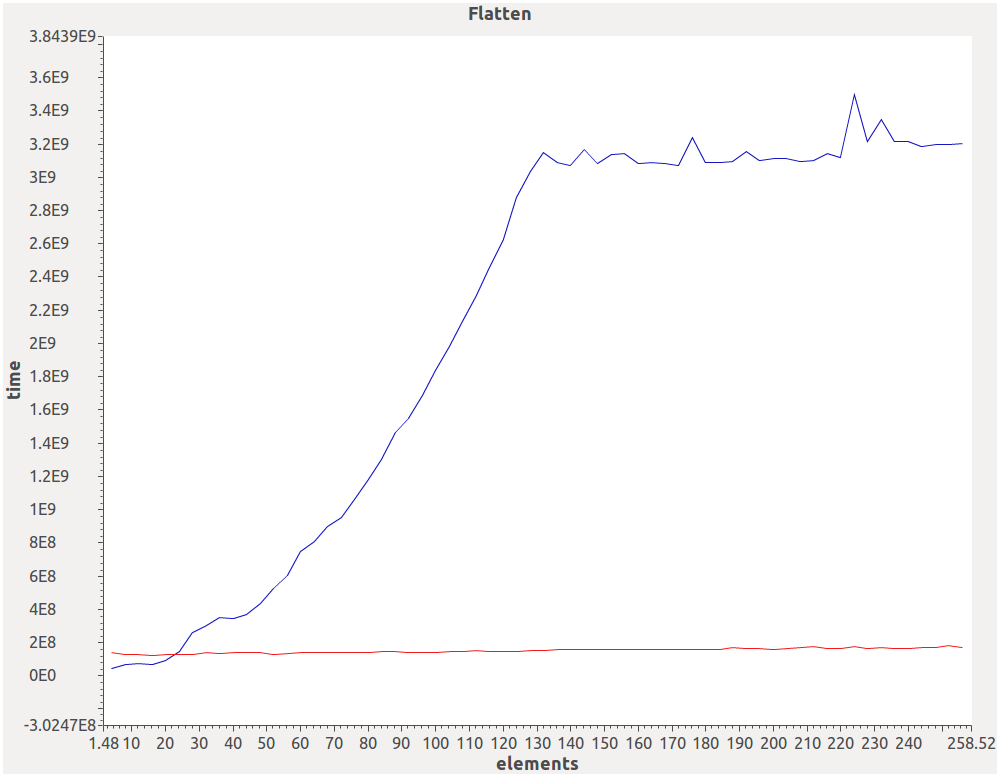
\includegraphics[width=\textwidth]{graphs/set/Flatten}
\end{figure*}
\pagebreak

\noindent\textbf{ForAll}
\lstinputlisting[firstline=1,lastline=3]{transformations/set/emftvm/TestForAll.atl}
\begin{figure*}[h]
\centering
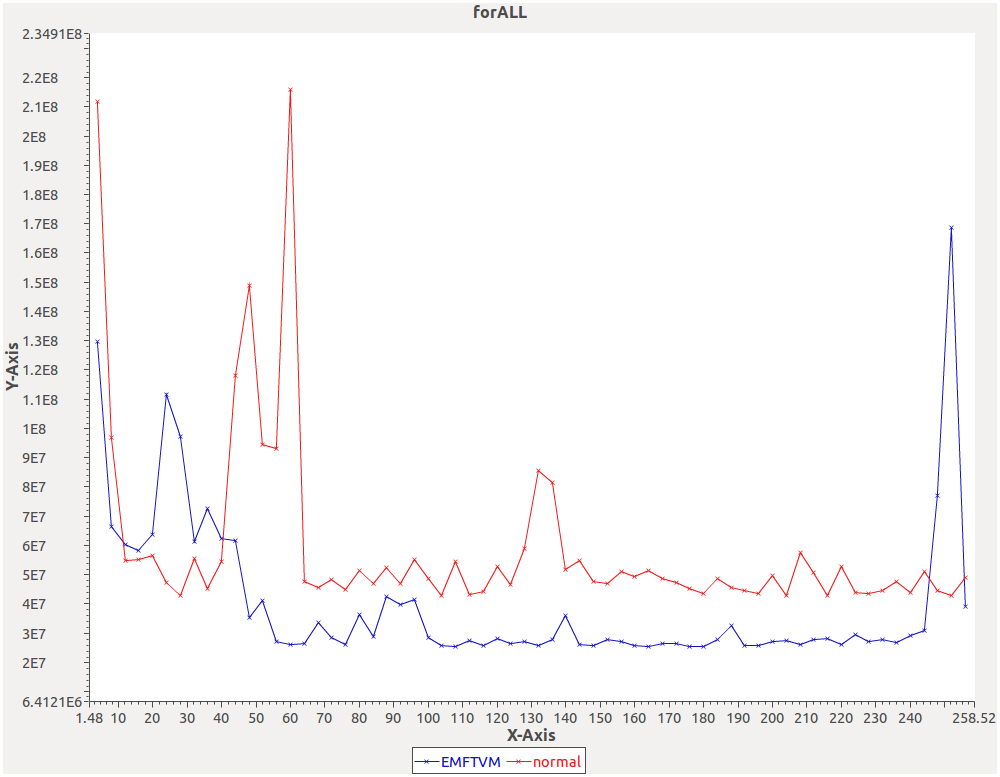
\includegraphics[width=\textwidth]{graphs/set/forALL}
\end{figure*}
\pagebreak

\noindent\textbf{Includes}
\lstinputlisting[firstline=1,lastline=3]{transformations/set/emftvm/TestIncludes.atl}
\begin{figure*}[h]
\centering
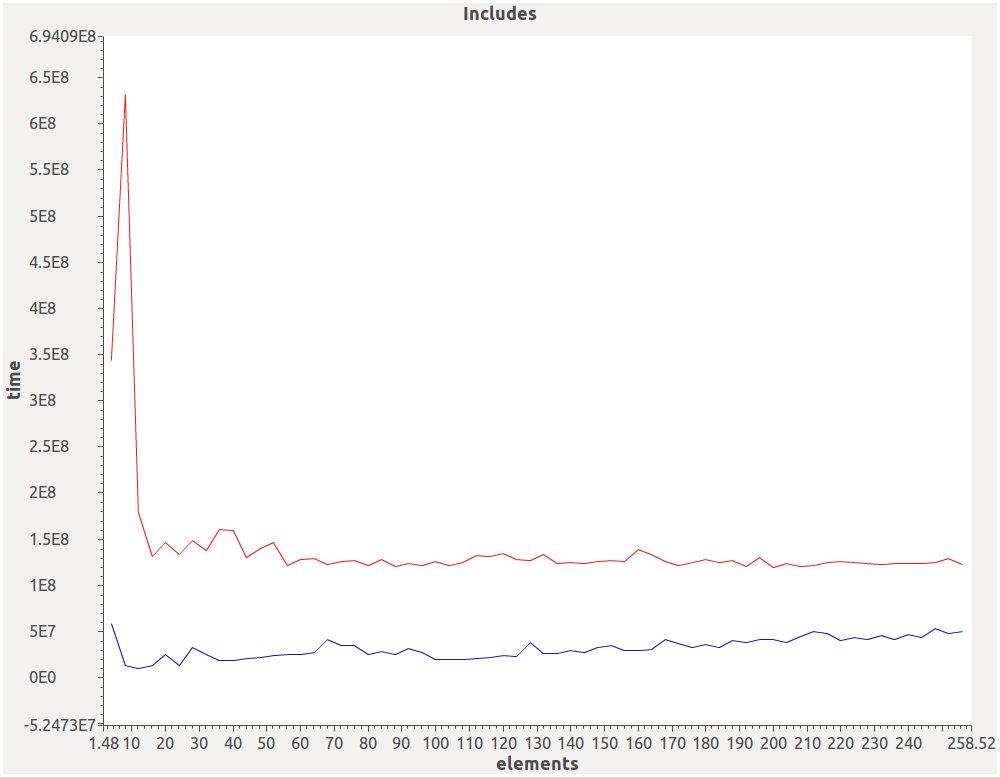
\includegraphics[width=\textwidth]{graphs/set/Includes}
\end{figure*}
\pagebreak

\noindent\textbf{IncludesAll}
\lstinputlisting[firstline=1,lastline=3]{transformations/set/emftvm/TestIncludesAll.atl}
\begin{figure*}[h]
\centering
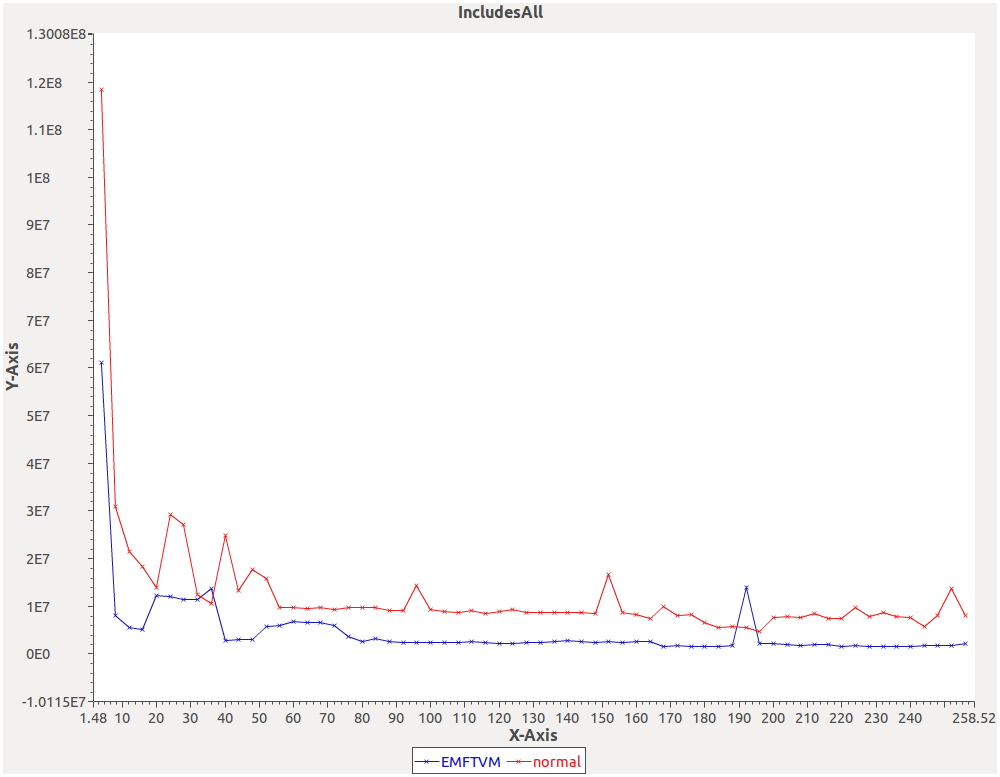
\includegraphics[width=\textwidth]{graphs/set/IncludesAll}
\end{figure*}
\pagebreak

\noindent\textbf{Including}
\lstinputlisting[firstline=1,lastline=3]{transformations/set/emftvm/TestIncluding.atl}
\begin{figure*}[h]
\centering
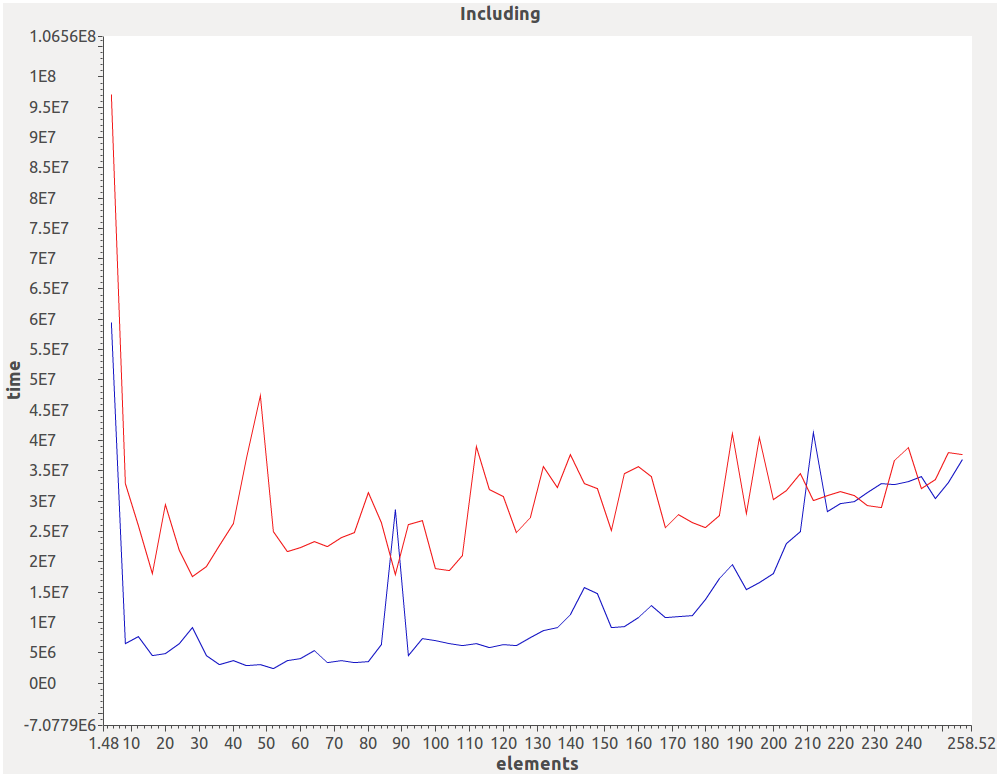
\includegraphics[width=\textwidth]{graphs/set/Including}
\end{figure*}
\pagebreak

\noindent\textbf{Intersection}
\lstinputlisting[firstline=1,lastline=3]{transformations/set/emftvm/TestIntersection.atl}
\begin{figure*}[h]
\centering
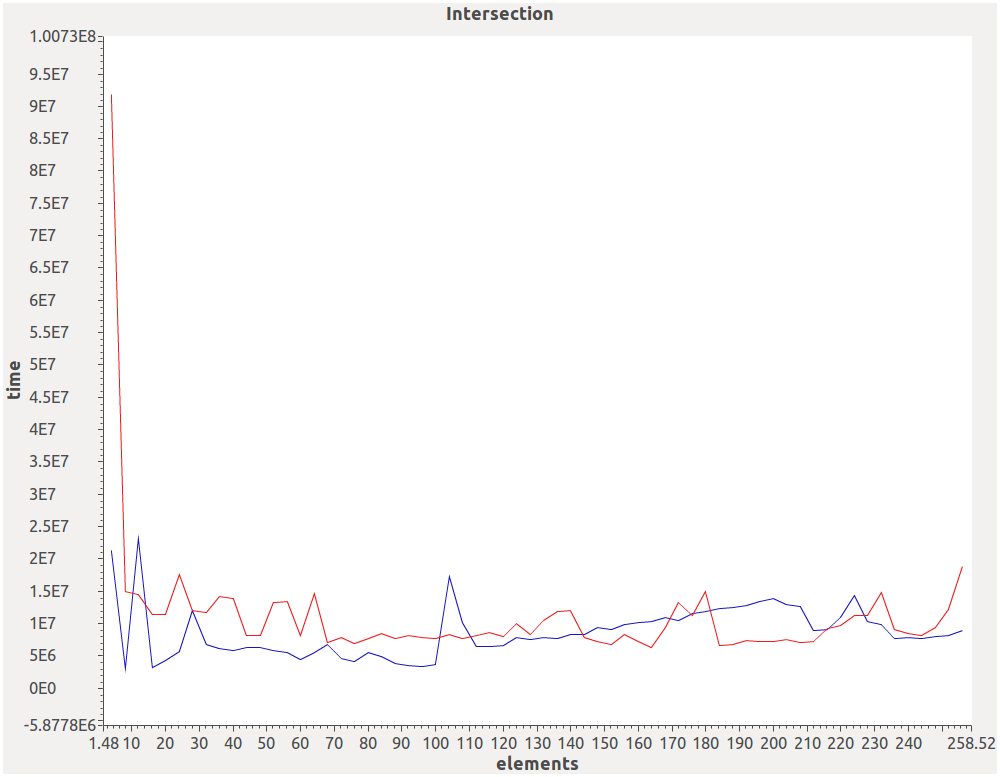
\includegraphics[width=\textwidth]{graphs/set/Intersection}
\end{figure*}
\pagebreak

\noindent\textbf{IsEmpty}
\lstinputlisting[firstline=1,lastline=3]{transformations/set/emftvm/TestIsEmpty.atl}
\begin{figure*}[h]
\centering
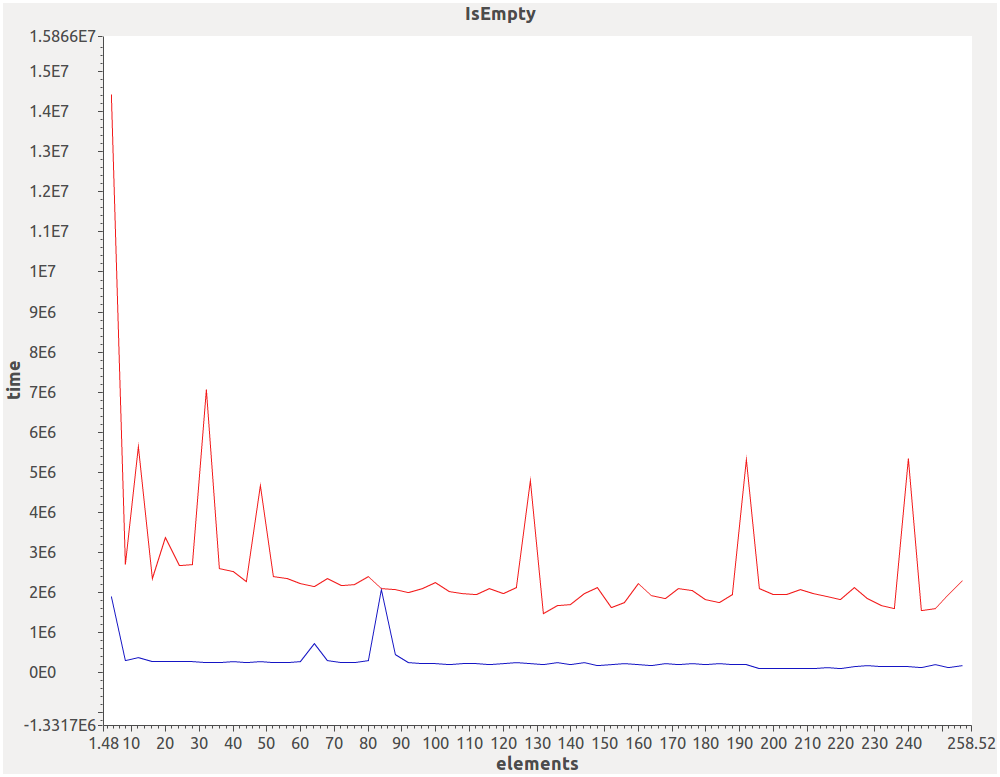
\includegraphics[width=\textwidth]{graphs/set/IsEmpty}
\end{figure*}
\pagebreak

\noindent\textbf{IsUnique}
\lstinputlisting[firstline=1,lastline=3]{transformations/set/emftvm/TestIsUnique.atl}
\begin{figure*}[h]
\centering
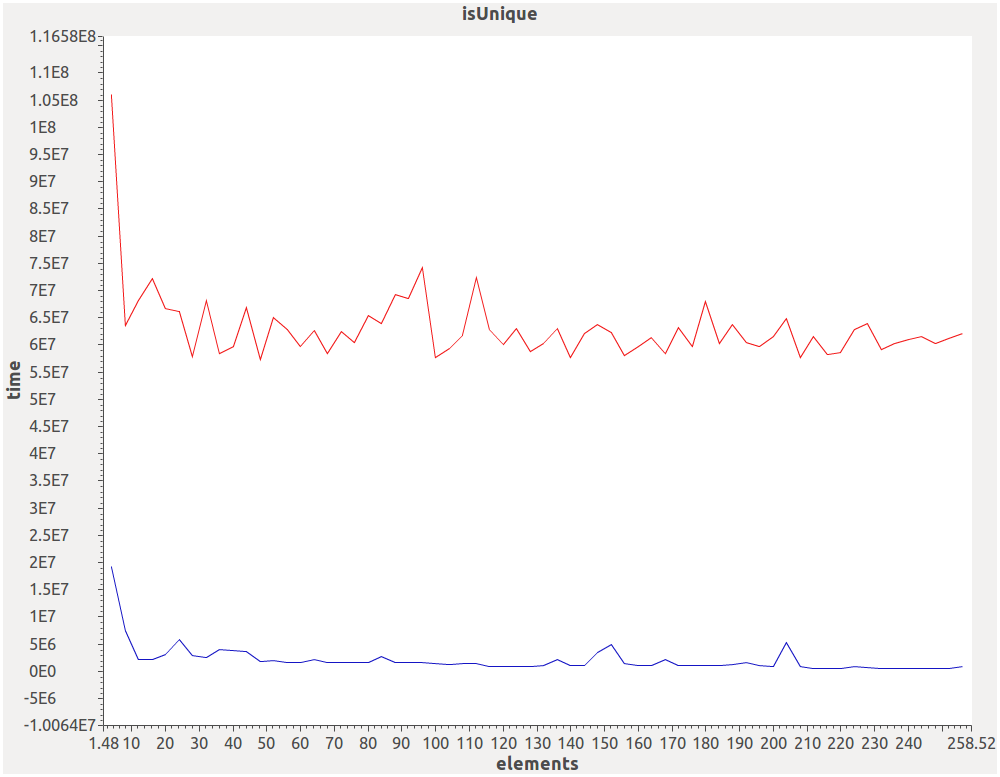
\includegraphics[width=\textwidth]{graphs/set/isUnique}
\end{figure*}
\pagebreak

\noindent\textbf{Iterate}
\lstinputlisting[firstline=1,lastline=3]{transformations/set/emftvm/TestIterate.atl}
\begin{figure*}[h]
\centering
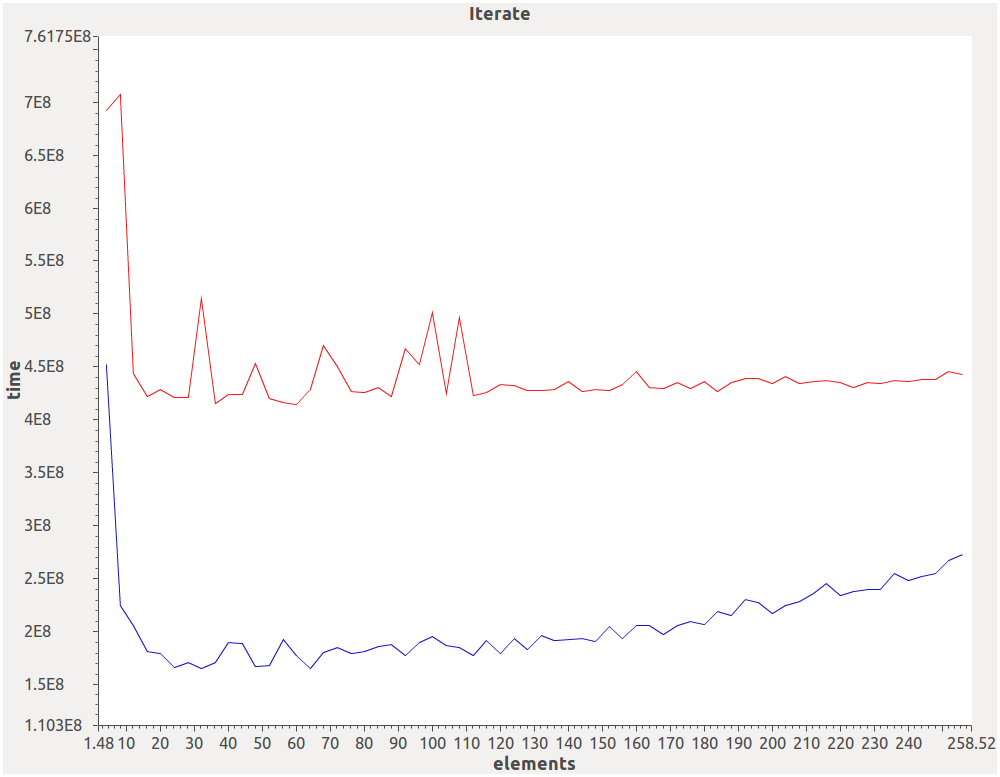
\includegraphics[width=\textwidth]{graphs/set/Iterate}
\end{figure*}
\pagebreak

\noindent\textbf{Minus}
\lstinputlisting[firstline=1,lastline=3]{transformations/set/emftvm/TestMinus.atl}
\begin{figure*}[h]
\centering
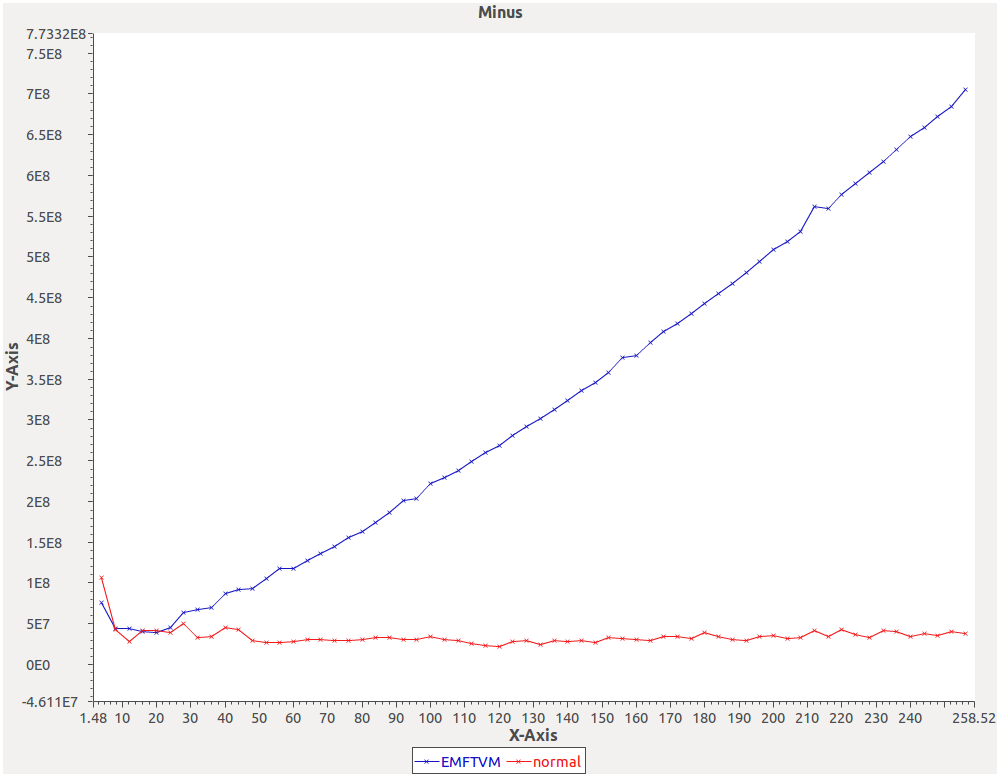
\includegraphics[width=\textwidth]{graphs/set/Minus}
\end{figure*}
\pagebreak

\noindent\textbf{NotEqual}
\lstinputlisting[firstline=1,lastline=3]{transformations/set/emftvm/TestNeq.atl}
\begin{figure*}[h]
\centering
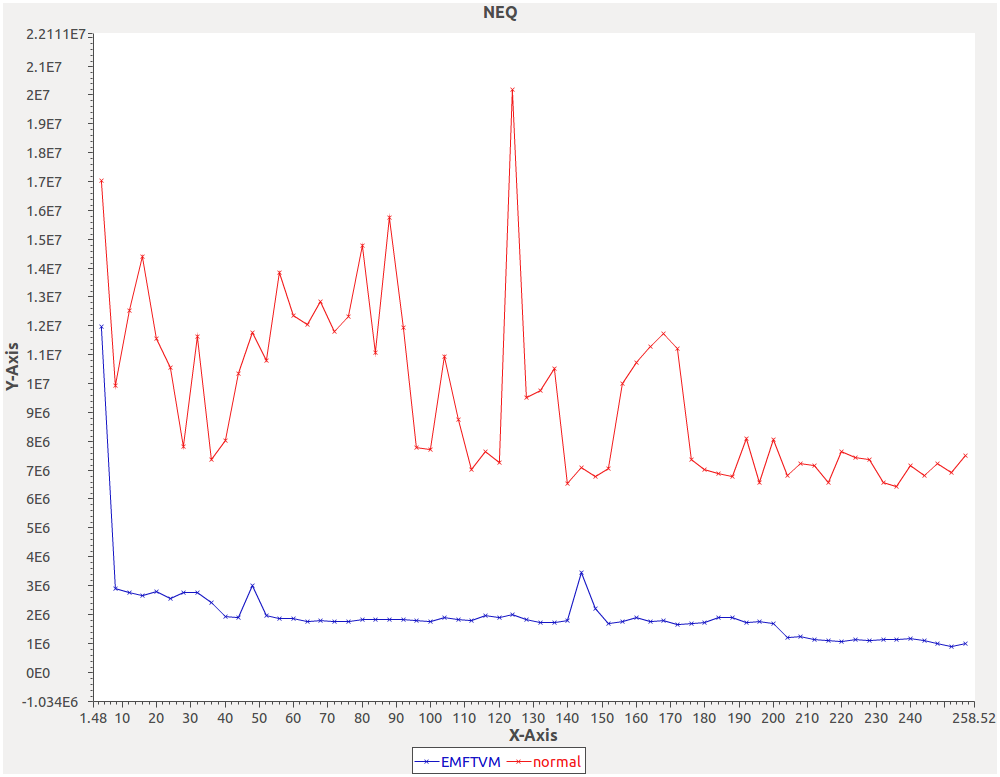
\includegraphics[width=\textwidth]{graphs/set/NEQ}
\end{figure*}
\pagebreak

\noindent\textbf{One}
\lstinputlisting[firstline=1,lastline=3]{transformations/set/emftvm/TestOne.atl}
\begin{figure*}[h]
\centering
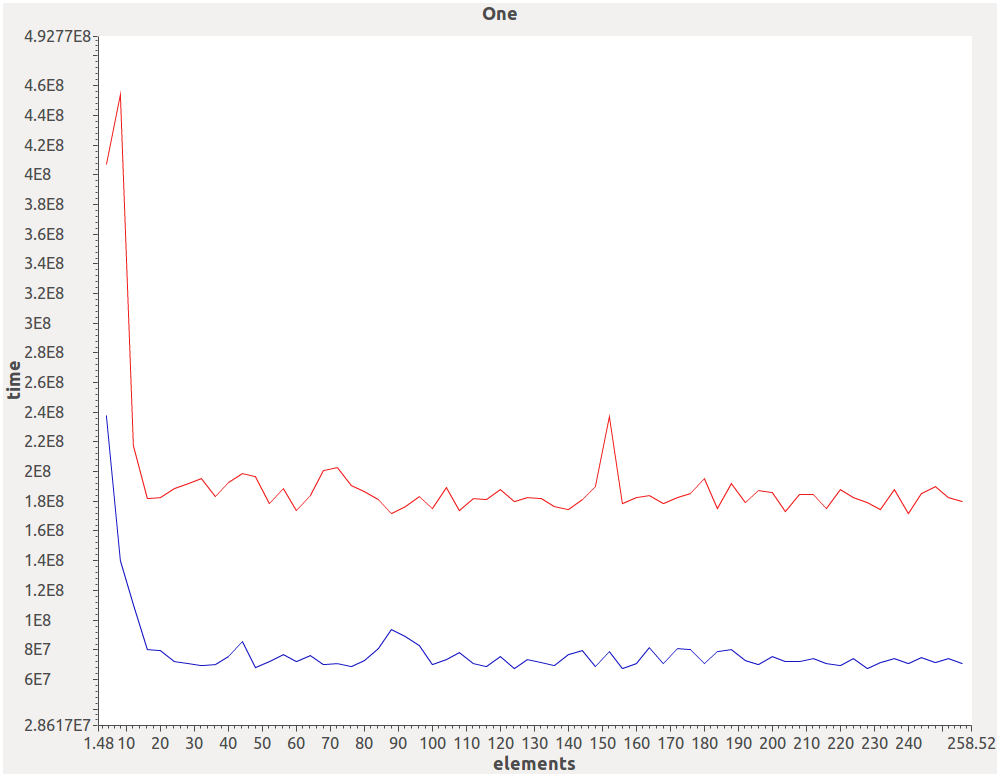
\includegraphics[width=\textwidth]{graphs/set/One}
\end{figure*}
\pagebreak

\noindent\textbf{Reject}
\lstinputlisting[firstline=1,lastline=3]{transformations/set/emftvm/TestReject.atl}
\begin{figure*}[h]
\centering
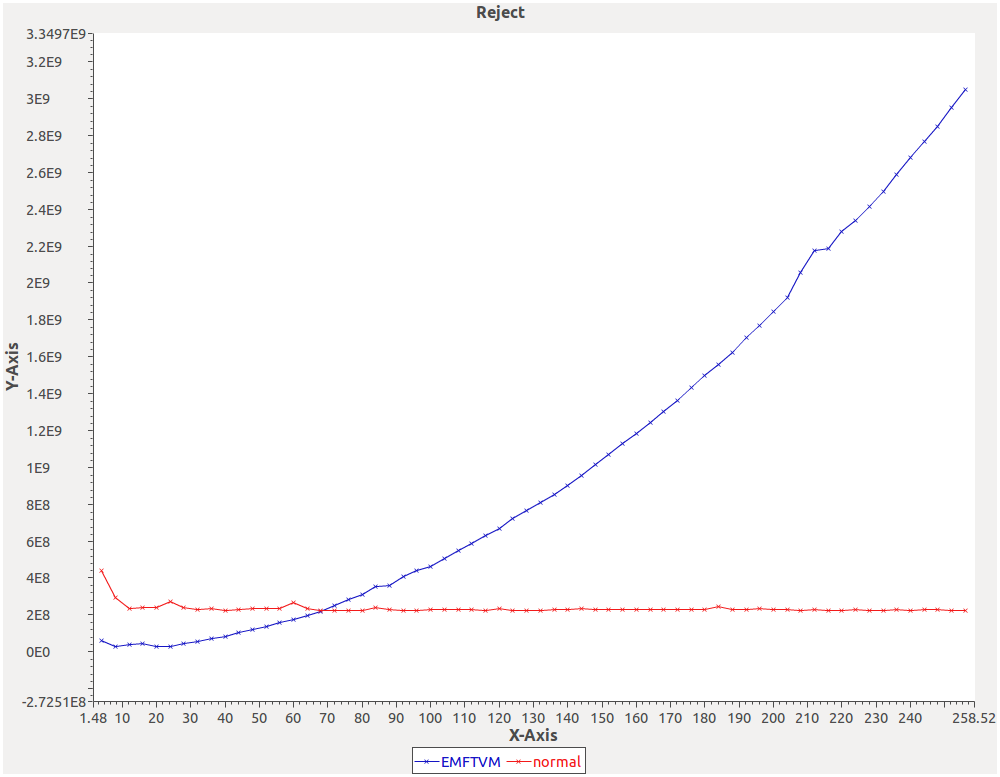
\includegraphics[width=\textwidth]{graphs/set/Reject}
\end{figure*}
\pagebreak

\noindent\textbf{Select}
\lstinputlisting[firstline=1,lastline=3]{transformations/set/emftvm/TestSelect.atl}
\begin{figure*}[h]
\centering
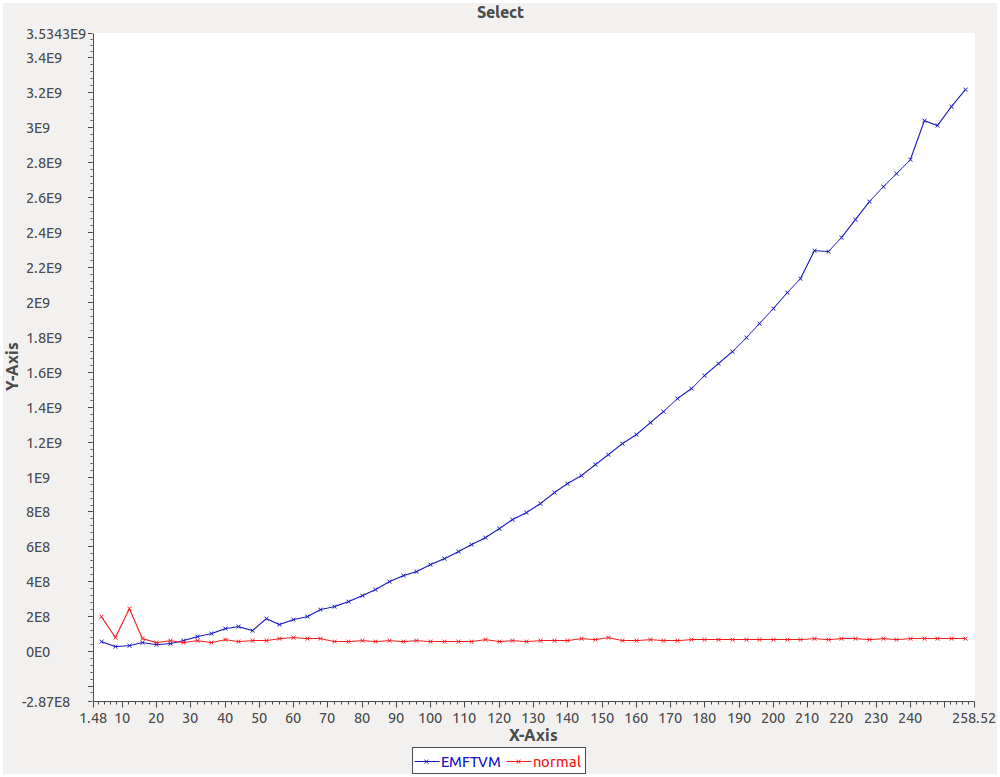
\includegraphics[width=\textwidth]{graphs/set/Select}
\end{figure*}
\pagebreak

\noindent\textbf{Size}
\lstinputlisting[firstline=1,lastline=3]{transformations/set/emftvm/TestSize.atl}
\begin{figure*}[h]
\centering
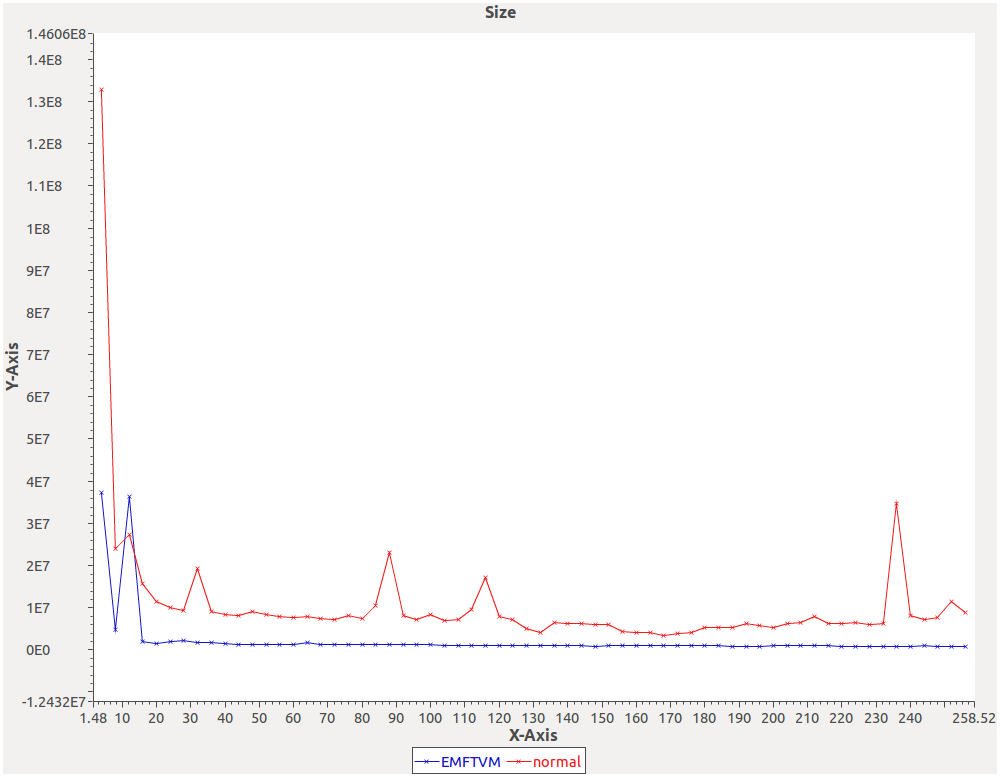
\includegraphics[width=\textwidth]{graphs/set/Size}
\end{figure*}
\pagebreak

\noindent\textbf{SortedBy}
\lstinputlisting[firstline=1,lastline=3]{transformations/set/emftvm/TestSortedBy.atl}
\begin{figure*}[h]
\centering
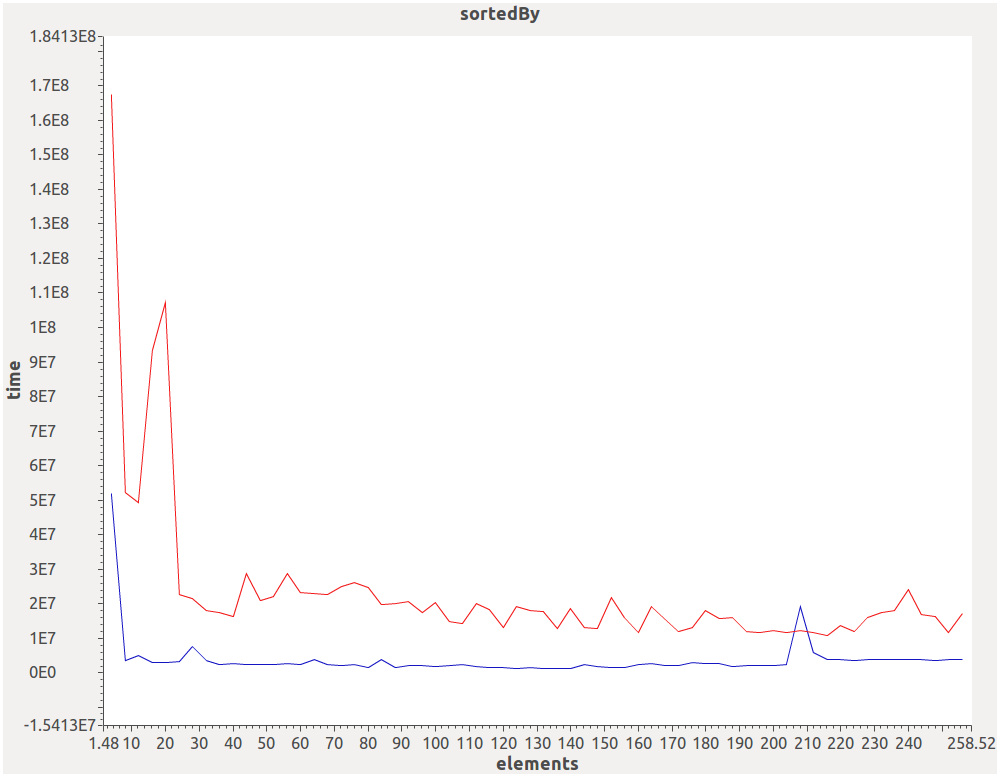
\includegraphics[width=\textwidth]{graphs/set/sortedBy}
\end{figure*}
\pagebreak

\noindent\textbf{Sum}
\lstinputlisting[firstline=1,lastline=3]{transformations/set/emftvm/TestSum.atl}
\begin{figure*}[h]
\centering
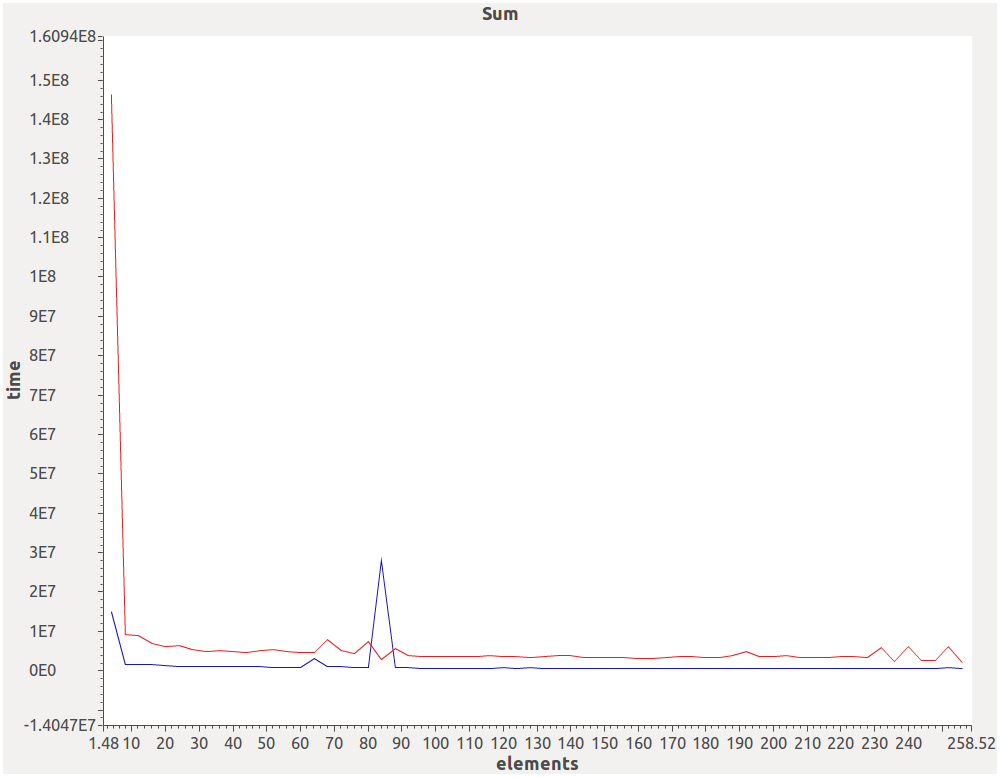
\includegraphics[width=\textwidth]{graphs/set/Sum}
\end{figure*}
\pagebreak

\noindent\textbf{SymmetricDif}
\lstinputlisting[firstline=1,lastline=3]{transformations/set/emftvm/TestSymmetricDif.atl}
\begin{figure*}[h]
\centering
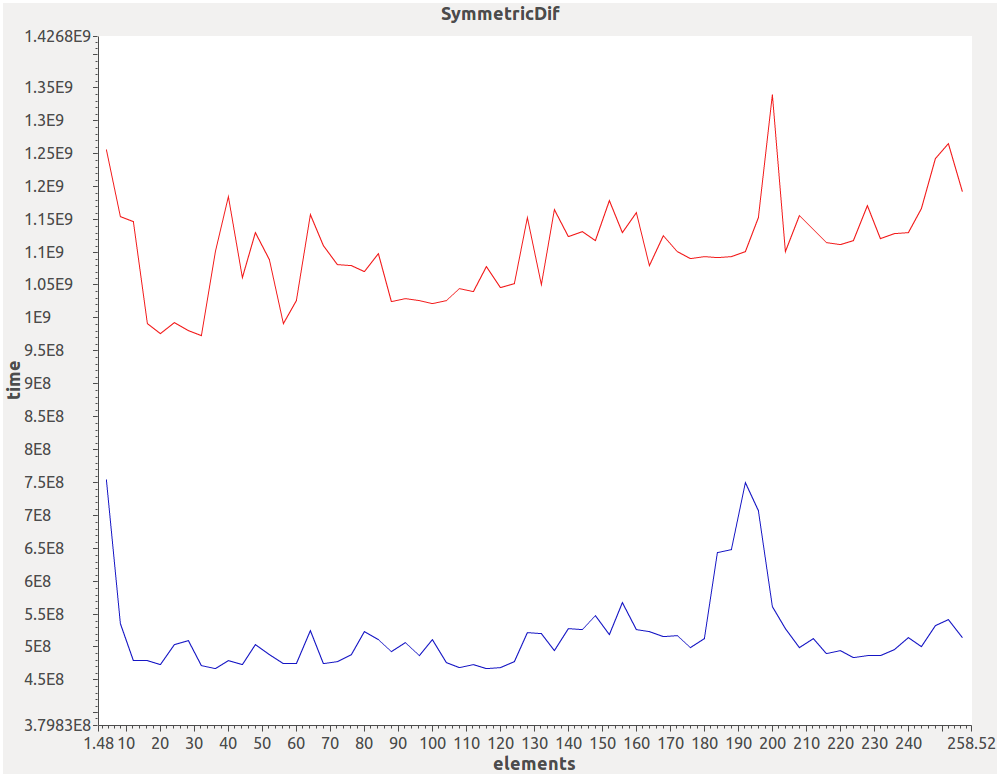
\includegraphics[width=\textwidth]{graphs/set/SymmetricDif}
\end{figure*}
\pagebreak

\noindent\textbf{Union}
\lstinputlisting[firstline=1,lastline=3]{transformations/set/emftvm/TestUnion.atl}
\begin{figure*}[h]
\centering
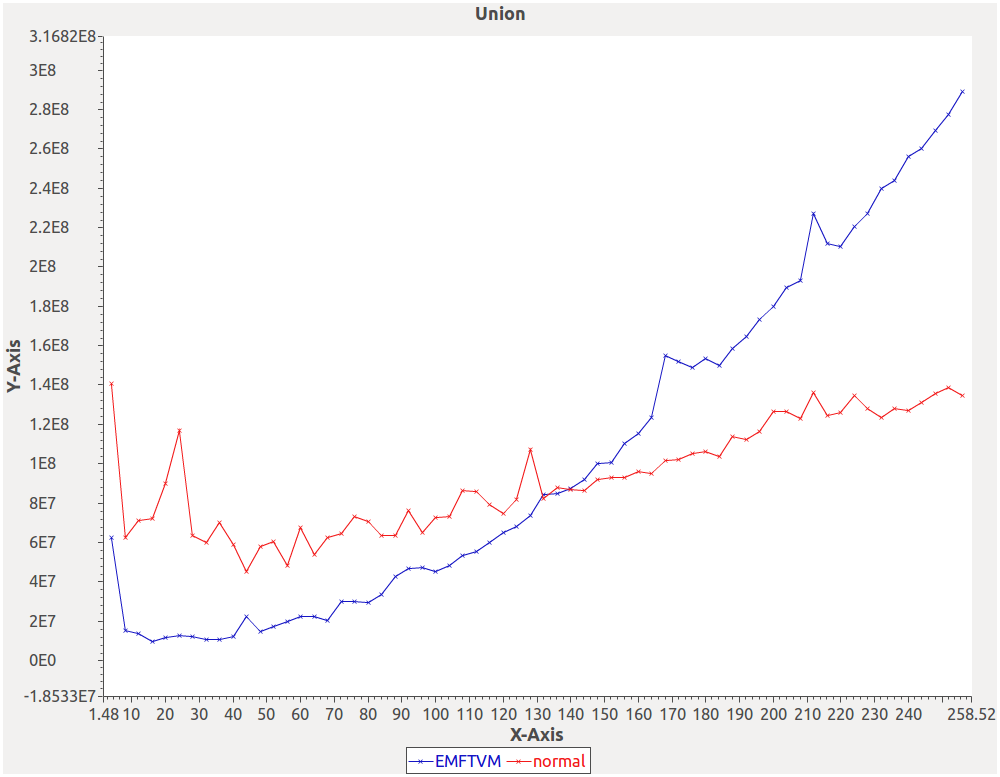
\includegraphics[width=\textwidth]{graphs/set/Union}
\end{figure*}
\pagebreak